

%\begin{sidewaysfigure}
%\centering
%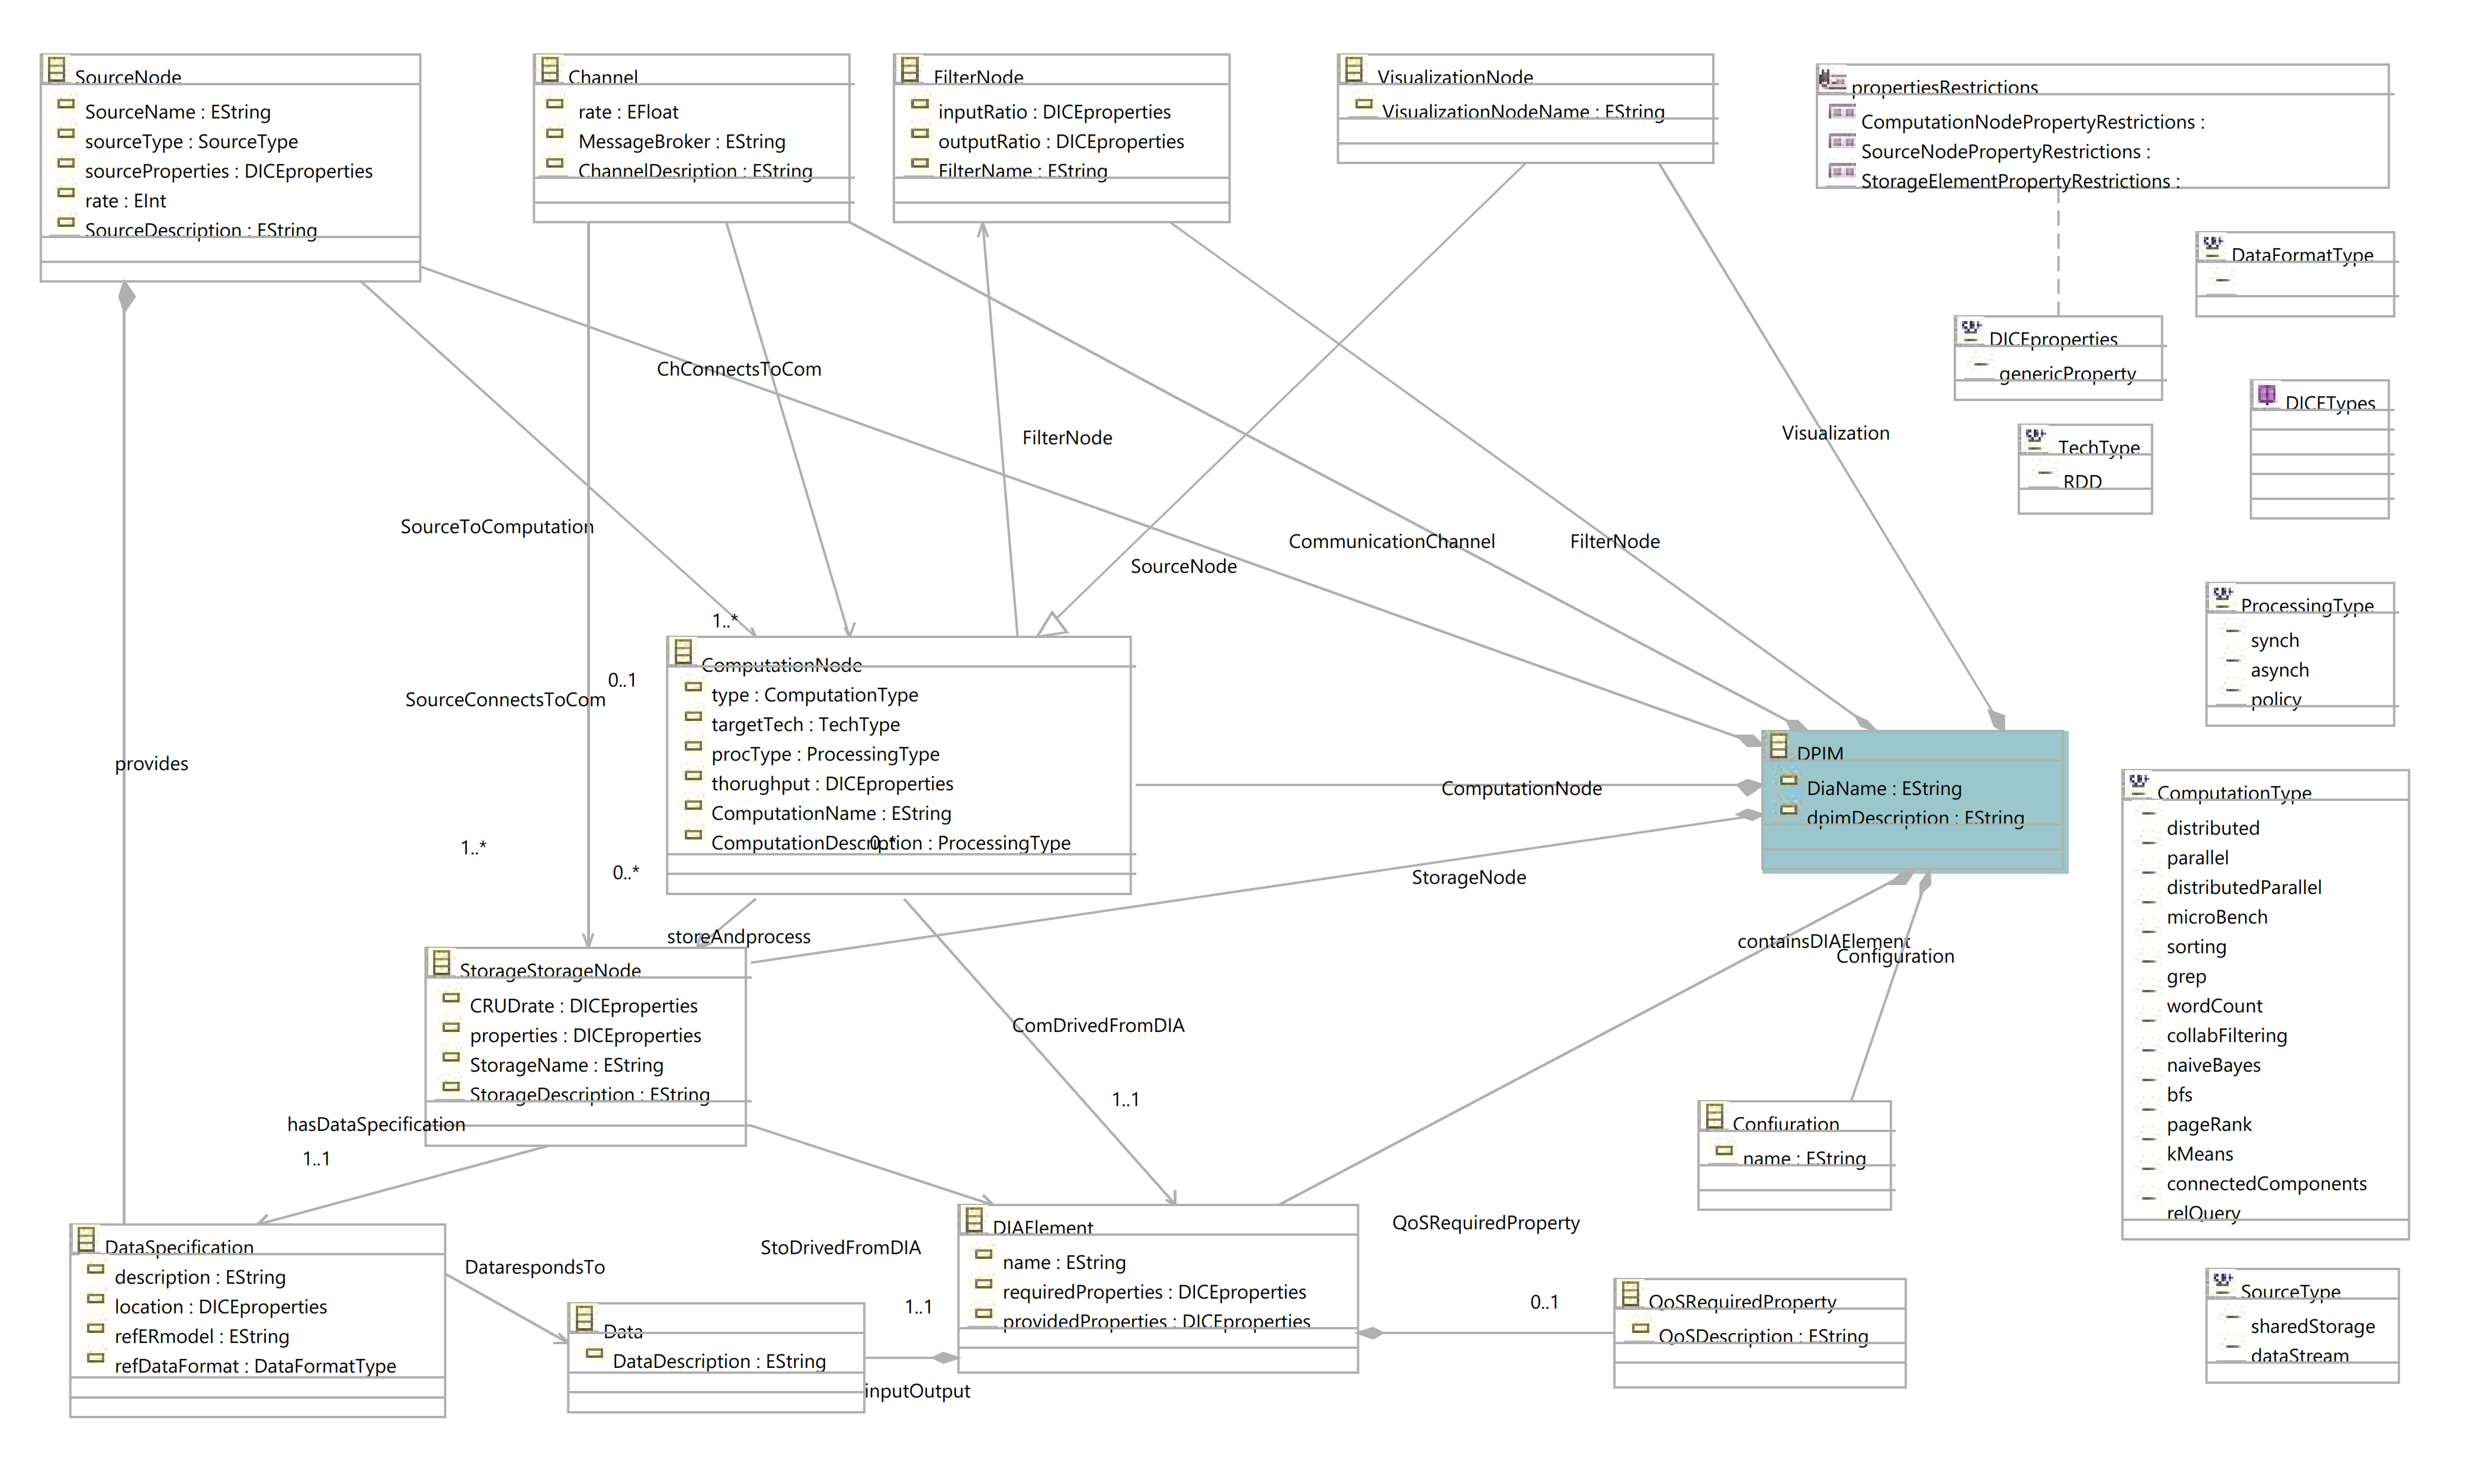
\includegraphics[width=\textwidth]{Images/11.png}
%\caption{\label{fig:metamodel}DICE DPIM metamodel.}
%\end{sidewaysfigure}

%\begin{figure}
%\centering
%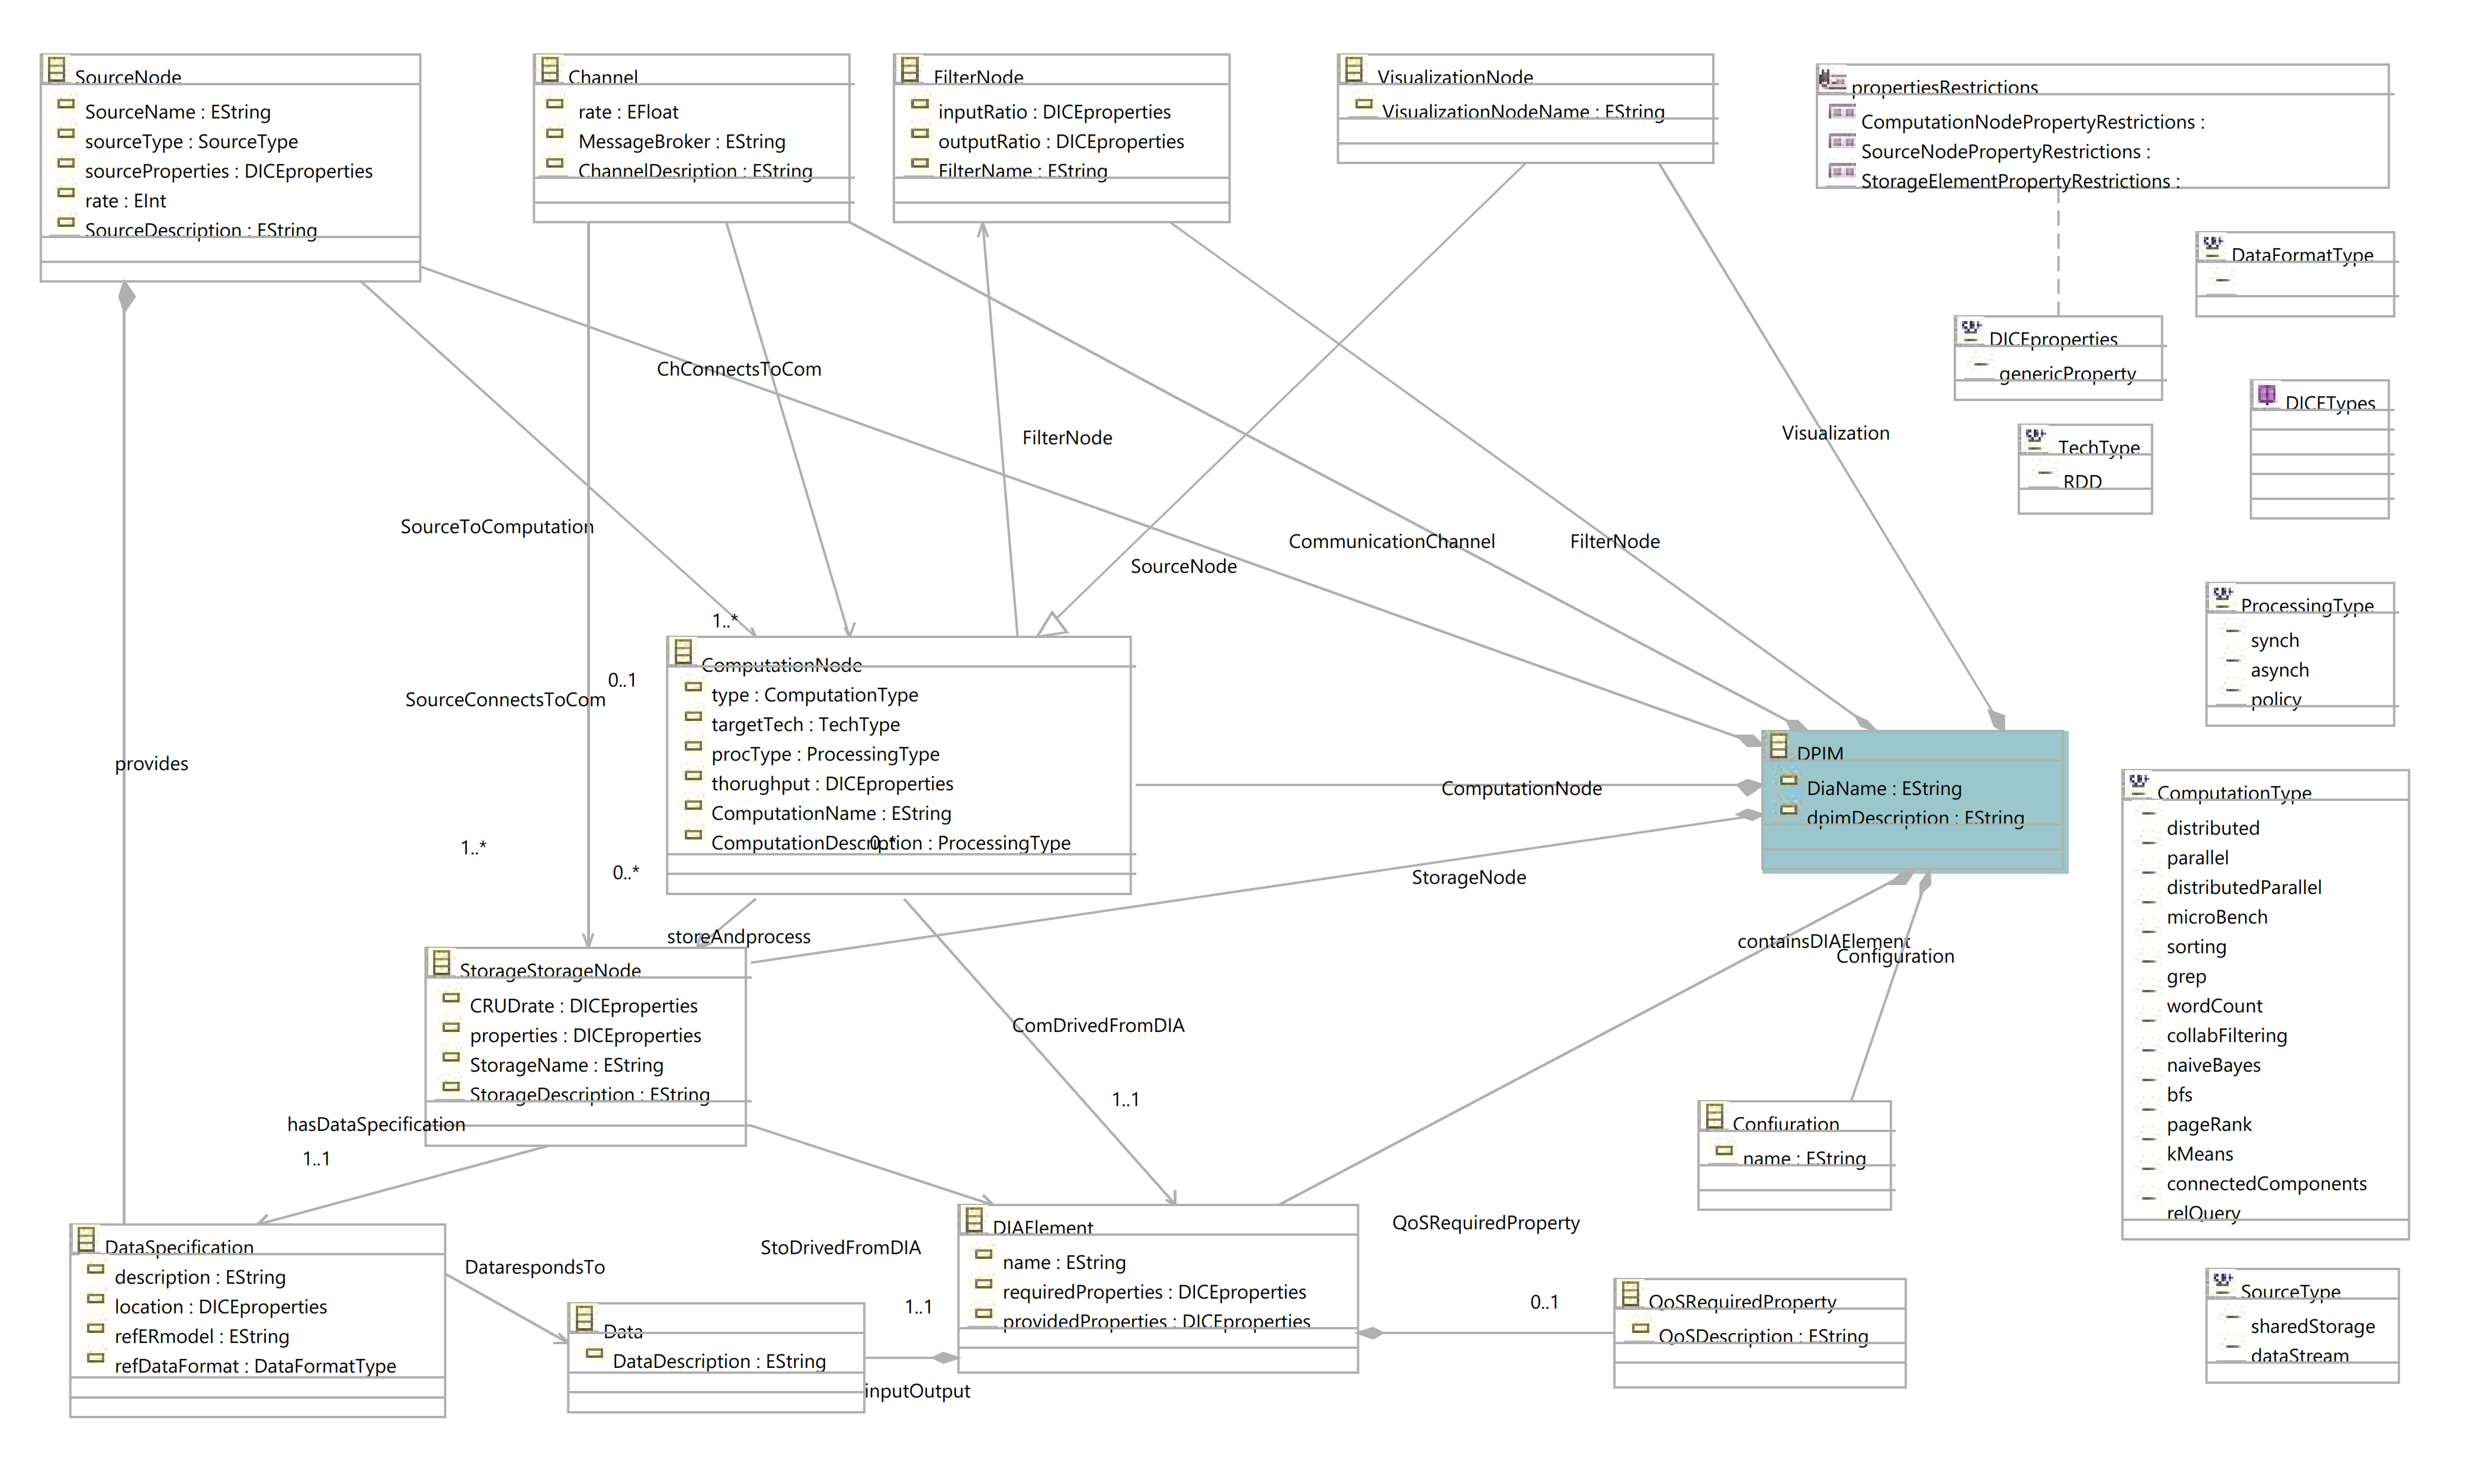
\includegraphics[width=\textwidth]{Images/11.png}
%\caption{\label{fig:metamodel2}DICE DPIM metamodel in portrait form.}
%\end{figure}

\subsection{Product perspective }


add here class diagram + verbal description



%add a state diagram for each subsect


\subsection{Product functions}

\subsubsection{login }
\subsubsection{sending pics}
\subsubsection{mining info }
\subsubsection{issue a ticket }
\subsubsection{generate statistics}

\subsection{User characteristics }


\subsection{Assumptions, dependencies and constraints}
\begin{enumerate}[label=D]
\item the device should acquire position with an accuracy of enouth meters in order to univocally determine the road (e.g. 5 meters)
\item the device should take pictures with enouth resolution to be able to read the licence plate using the algorithm
\item in every picture the licence plate should be visible and the kind of violation
\item the number and kind of violation should be finite (defined by the law)
\item every authority account is verified and it's not possible to be created using the frontend
\
\end{enumerate}
